\documentclass[11pt,a4paper]{article}

\usepackage[utf8]{inputenc}
\usepackage[T1]{fontenc}
\usepackage[spanish]{babel}
\usepackage{csquotes}
\usepackage[
    a4paper,
    margin=2.5cm,
    includeheadfoot,
    headheight=14pt,
    headsep=0.6cm,
    footskip=0.9cm
]{geometry}

\usepackage{lmodern}
\usepackage[table]{xcolor}
\usepackage{array}
\usepackage{tabularx}
\usepackage{longtable}
\usepackage{booktabs}
\usepackage{graphicx}
\usepackage{enumitem}
\usepackage{fancyhdr}
\usepackage{titlesec}
\usepackage[backend=biber,style=ieee,sorting=none]{biblatex}

\addbibresource{referencias/referencias.bib}

\usepackage[hidelinks]{hyperref}

\definecolor{azul}{HTML}{17365D}
\definecolor{azulclaro}{HTML}{EDF2F7}

\setlength{\parindent}{0pt}
\setlength{\parskip}{5pt}
\setlength{\tabcolsep}{8pt}
\renewcommand{\arraystretch}{1.35}

\setlist[itemize]{leftmargin=*,itemsep=4pt}
\setlist[enumerate]{leftmargin=*,itemsep=4pt}

\titleformat{\section}
    {\large\bfseries\color{azul}}
    {\thesection.}{0.6em}{}

\titleformat{\subsection}
    {\normalsize\bfseries}
    {\thesubsection.}{0.6em}{}

\titlespacing*{\section}{0pt}{12pt}{5pt}
\titlespacing*{\subsection}{0pt}{8pt}{3pt}

\setcounter{tocdepth}{2}

\addto\captionsspanish{
    \renewcommand{\contentsname}{Índice de contenido}
}

\pagestyle{fancy}
\fancyhf{}

\fancyhead[L]{\small UTEQ · Ingeniería de Requerimientos}
\fancyhead[R]{\small TA-PFC-E1}

\fancyfoot[L]{\footnotesize Equipo CERY}
\fancyfoot[R]{\footnotesize Página \thepage}

\renewcommand{\headrulewidth}{0.4pt}
\renewcommand{\footrulewidth}{0.4pt}

\raggedbottom

\begin{document}

\begin{titlepage}

\thispagestyle{empty}

\begin{center}

\vspace*{0.2cm}

{\large\bfseries
UNIVERSIDAD TÉCNICA ESTATAL DE QUEVEDO}

\vspace{0.35cm}

Facultad de Ciencias de la Computación

Carrera de Ingeniería de Software

\vspace{0.45cm}

{\color{azul}\rule{\textwidth}{1pt}}

\vspace{0.45cm}

{\large\bfseries PROYECTO FIN DE CURSO}

\vspace{0.25cm}

{\large\bfseries TA-PFC-E1}

\vspace{0.4cm}

{\Large\bfseries
Sistema de gestión de tutorías y seguimiento estudiantil}

\vspace{0.35cm}

{\large
Entrega 1: visión, alcance, partes interesadas,
contexto y plan de elicitación}

\vspace{0.6cm}

\end{center}

\arrayrulecolor{azul}

\begin{tabularx}{\textwidth}{
    |>{\columncolor{azulclaro}\raggedright\arraybackslash}p{3.6cm}
    |>{\raggedright\arraybackslash}X|
}

\hline

\rowcolor{azul}
\textcolor{white}{\textbf{Campo}} &
\textcolor{white}{\textbf{Detalle}} \\

\hline

Integrantes &
Angelo Maximiliano Espinoza Pivaque \newline
Luis Antonio Yepez Guagua \newline
Jordy Fabián Rivas Bodero \newline
Yerai David Chalacán Toala \\

\hline

Asignatura &
Ingeniería de Requerimientos (ISR-401) \\

\hline

Nivel y paralelo &
Cuarto nivel · Paralelo A \\

\hline

Docente &
Gleiston Cicerón Guerrero Ulloa, PhD \\

\hline

Modalidad &
Trabajo autónomo grupal con calificación individual \\

\hline

Fecha límite &
21 de noviembre de 2026, 23:59 \\

\hline

Período &
2026--2027 SPA \\

\hline

\end{tabularx}

\vfill

\begin{center}

{\color{azul}\rule{\textwidth}{1pt}}

Quevedo -- Ecuador

2026

\end{center}

\end{titlepage}

\pagenumbering{roman}

\tableofcontents

\clearpage

\pagenumbering{arabic}

\section{Organización y planteamiento del problema}

\subsection{Identificación de la organización}

\subsection{Contacto inicial y aceptación de la organización}

\subsection{Descripción del proceso actual y problemática}

En el proceso inicialmente descrito para las tutorías académicas, los estudiantes se acercan presencialmente al docente para comunicar las dificultades que presentan y los temas en los que necesitan refuerzo. Una vez acordada la realización de una tutoría, la coordinación continúa mediante WhatsApp, donde se establece la fecha y la hora, se confirma la sesión y se notifican posibles cambios.

Esta forma de organización hace que la información quede repartida entre conversaciones presenciales y mensajes. Las solicitudes, propuestas de horarios y confirmaciones no se encuentran reunidas en un mismo lugar. Por ello, cuando se presentan modificaciones o existen varias propuestas, los participantes deben revisar las conversaciones para identificar cuál es el horario definitivo y qué solicitudes todavía están pendientes.

Otro aspecto que merece atención es la continuidad del acompañamiento académico. Para preparar una nueva sesión, el docente necesita conocer qué temas se trataron anteriormente, qué recomendaciones recibió el estudiante y qué actividades quedaron pendientes. Cuando estos antecedentes se encuentran en mensajes o apuntes separados, recuperarlos requiere consultar distintas fuentes. Esto puede dificultar el seguimiento de los avances y la continuidad del trabajo realizado en tutorías anteriores.

A esta situación se suma la necesidad de conocer cómo evoluciona el rendimiento académico de los estudiantes. El seguimiento no debería limitarse al registro de las sesiones realizadas, sino que también debe permitir reconocer si las dificultades identificadas persisten y si es necesario ofrecer apoyo adicional. Sin embargo, todavía es necesario conocer qué información utilizan los docentes para realizar este seguimiento, de dónde provienen los datos y qué indicadores consideran relevantes para identificar posibles dificultades.

Estos aspectos se revisarán durante la elicitación con los participantes de la organización. También será necesario confirmar qué información está disponible, quiénes pueden consultarla y bajo qué condiciones podría utilizarse dentro del sistema.

En este contexto, el problema identificado inicialmente se relaciona con la dispersión de la información necesaria para organizar las tutorías y dar continuidad al acompañamiento académico. Aunque esta situación permite establecer una primera aproximación a las necesidades del sistema, será necesario contrastarla con estudiantes y docentes para conocer con mayor precisión la frecuencia de estas dificultades, sus consecuencias y los aspectos que requieren mayor atención.

\paragraph{Personas afectadas por la problemática.}

Los estudiantes necesitan conocer cuándo se realizarán sus tutorías y cuáles son los compromisos establecidos durante cada sesión. También requieren tener a disposición las recomendaciones recibidas y las actividades que deben desarrollar. Cuando esta información queda distribuida en diferentes conversaciones, pueden surgir dudas sobre los horarios acordados o perderse de vista algunas actividades pendientes.

Por su parte, los docentes tutores necesitan consultar los antecedentes de cada estudiante antes de continuar con el acompañamiento. Esto incluye los temas revisados, las recomendaciones realizadas y las dificultades que todavía requieren atención. Tener que recuperar estos datos desde mensajes y apuntes independientes puede aumentar el tiempo destinado a la organización de las sesiones.

La coordinación académica también se considera una parte interesada potencial, especialmente por su posible participación en la supervisión del proceso tutorial. No obstante, sus responsabilidades, necesidades de información y atribuciones dentro del sistema deberán confirmarse durante la elicitación.

\subsection{Fuentes y respaldo del diagnóstico}

\section{Visión y objetivos}

\subsection{Declaración de visión}

Para los estudiantes, los docentes tutores y la coordinación académica que necesitan organizar y dar seguimiento a las tutorías, se propone un sistema de gestión de tutorías y seguimiento estudiantil que reúna en un solo lugar las solicitudes, los horarios confirmados, las recomendaciones y las actividades pendientes de cada tutoría. A diferencia del proceso actual, que se apoya en conversaciones presenciales y mensajes de WhatsApp, el sistema busca que cada paso quede registrado y pueda consultarse por quien corresponda. Esta visión es una propuesta del equipo y se confirmará con la organización.


\subsection{Objetivos de negocio medibles}

Los objetivos de la Tabla~\ref{tab:objetivos} son propuestas del equipo. Todavía no existe una línea base: se obtendrá con la medición indicada en cada fila, y las metas quedan por acordar con la organización.

\begin{table}[ht]
\centering
\small
\caption{Objetivos de negocio medibles (propuestas por acordar).}
\label{tab:objetivos}
\begin{tabularx}{\textwidth}{|l|X|X|X|X|}
\hline
\textbf{ID} & \textbf{Resultado buscado} & \textbf{Indicador (unidad)} & \textbf{Línea base} & \textbf{Meta y plazo} \\ \hline
OBJ-01 & Reducir la espera entre la solicitud de una tutoría y su confirmación & Tiempo de confirmación (horas) & Por medir: registrar las solicitudes durante dos semanas & Por acordar; evaluación en la semana 17 \\ \hline
OBJ-02 & Aumentar las tutorías que quedan registradas con tema y asistencia & Proporción de tutorías con registro completo (\%) & Por medir: contar tutorías realizadas frente a registradas en un periodo & Por acordar; evaluación en la semana 17 \\ \hline
OBJ-03 & Reducir el tiempo para reunir el historial de tutorías de un estudiante & Tiempo de consulta del historial (minutos) & Por medir: cronometrar la consulta actual en varios casos & Por acordar; evaluación en la semana 17 \\ \hline
\end{tabularx}
\end{table}


\subsection{Criterios de medición de los objetivos}

Cada indicador se mide con registros que el equipo pueda revisar. El tiempo de confirmación (OBJ-01) se toma de la fecha y hora de la solicitud y de la confirmación. La proporción de tutorías registradas (OBJ-02) se calcula dividiendo las tutorías con tema y asistencia registrados entre las tutorías realizadas en el periodo. El tiempo de consulta del historial (OBJ-03) se cronometra en varios casos reales. La medición la realizará el equipo junto con la coordinación académica, y las metas se fijarán solo cuando exista la línea base. Los indicadores apoyan la revisión académica; no se afirma capacidad predictiva ni diagnóstico concluyente.


\section{Alcance y restricciones}

\subsection{Procesos incluidos en el sistema}

\subsection{Procesos excluidos del proyecto}

\subsection{Restricciones conocidas}

\subsection{Supuestos y aspectos por confirmar}

\section{Partes interesadas}

\subsection{Identificación de roles}

Las partes interesadas se identifican por rol y no por nombre. Hasta ahora se han confirmado tres roles: estudiante, docente tutor y coordinación académica. Los demás roles de la Tabla~\ref{tab:stakeholders} son candidatos del equipo y están marcados como \textit{propuesto}, a la espera de confirmarse con la organización. La identificación de las partes interesadas es una práctica reconocida de la gestión de proyectos \cite{pmbok2021}, y la norma ISO/IEC/IEEE 29148 distingue las necesidades de las partes interesadas de los requisitos del sistema y del software \cite{iso29148}.

\begin{table}[ht]
\centering
\small
\caption{Partes interesadas por rol.}
\label{tab:stakeholders}
\begin{tabularx}{\textwidth}{|l|l|X|l|}
\hline
\textbf{ID} & \textbf{Rol} & \textbf{Qué necesita del sistema} & \textbf{Estado} \\ \hline
SH-01 & Estudiante & Solicitar tutorías y consultar su seguimiento & Confirmado \\ \hline
SH-02 & Docente tutor & Registrar tutorías y consultar antecedentes & Confirmado \\ \hline
SH-03 & Coordinación académica & Ver el seguimiento y la continuidad de las tutorías & Confirmado \\ \hline
SH-04 & Autoridad de la unidad académica & Que el proyecto cumpla los procesos de la unidad & Propuesto \\ \hline
SH-05 & Administración técnica (TI) & Que el sistema sea mantenible y compatible con su entorno & Propuesto \\ \hline
SH-06 & Responsable de datos académicos & Controlar qué datos de los estudiantes se usan & Propuesto \\ \hline
SH-07 & Apoyo o bienestar estudiantil & Recibir alertas de estudiantes que lo necesiten & Propuesto \\ \hline
SH-08 & Responsable de protección de datos & Que el tratamiento de datos personales sea adecuado & Propuesto \\ \hline
\end{tabularx}
\end{table}


\subsection{Interés, influencia y disponibilidad}

La Tabla~\ref{tab:influencia} resume la valoración de cada rol. Todas las valoraciones son propuestas del equipo, y la disponibilidad se mantiene por confirmar; para cada rol propuesto se indica quién la consultará.

\begin{table}[ht]
\centering
\small
\caption{Interés, influencia y disponibilidad (propuestas por confirmar).}
\label{tab:influencia}
\begin{tabularx}{\textwidth}{|l|l|l|X|}
\hline
\textbf{ID} & \textbf{Interés} & \textbf{Influencia} & \textbf{Disponibilidad} \\ \hline
SH-01 & Alto & Baja & Por confirmar \\ \hline
SH-02 & Alto & Media & Por confirmar \\ \hline
SH-03 & Alto & Alta & Por confirmar \\ \hline
SH-04 & Medio & Alta & Por confirmar con la coordinación \\ \hline
SH-05 & Medio & Media & Por confirmar con la coordinación \\ \hline
SH-06 & Medio & Media & Por confirmar con la coordinación \\ \hline
SH-07 & Medio & Baja & Por confirmar con la coordinación \\ \hline
SH-08 & Bajo & Alta & Por confirmar con la coordinación \\ \hline
\end{tabularx}
\end{table}


\subsection{Matriz poder--interés}

La Figura~\ref{fig:matriz} ubica a los ocho roles según su poder y su interés. El archivo editable está en \texttt{modelos/matriz\_poder\_interes.drawio}.

\begin{figure}[ht]
\centering
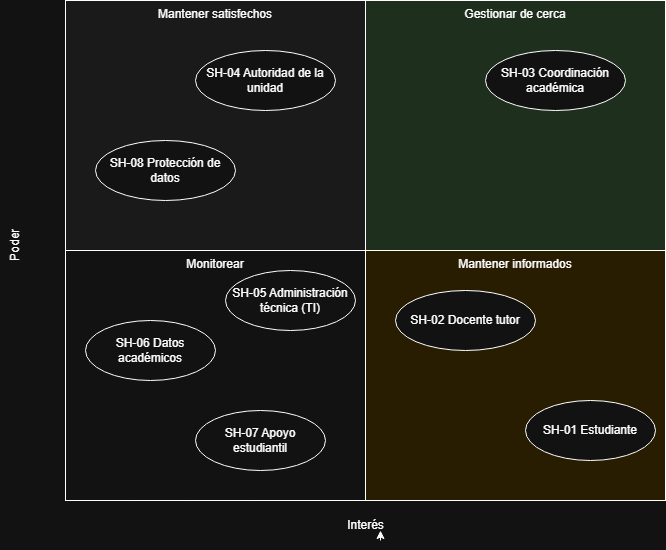
\includegraphics[width=0.85\textwidth,height=0.45\textheight,keepaspectratio]{figuras/matriz_poder_interes.png}
\caption{Matriz poder--interés de las partes interesadas.}
\label{fig:matriz}
\end{figure}


\subsection{Estrategias de participación}

Para los roles de poder alto e interés alto (SH-03) se propone gestionar de cerca, con reuniones para acordar el alcance. Para los de poder alto e interés medio o bajo (SH-04 y SH-08) se propone mantenerlos satisfechos, consultándolos solo sobre autorizaciones y protección de datos. Para los de interés alto y poder bajo o medio (SH-01 y SH-02) se propone mantenerlos informados mediante entrevistas y validación de lo documentado. Para los demás (SH-05, SH-06 y SH-07) se propone monitorear con consultas puntuales. La técnica y la frecuencia de cada contacto se detallan en el plan de elicitación.


\section{Contexto del sistema}

\subsection{Límite del sistema y entidades externas}

El sistema de gestión de tutorías y seguimiento estudiantil contempla el registro y la consulta de solicitudes, horarios confirmados, acuerdos, recomendaciones y actividades relacionadas con las tutorías. También considera el seguimiento de los estudiantes mediante indicadores de rendimiento académico, cuya disponibilidad y forma de utilización deberán definirse durante el levantamiento de requisitos.

Dentro de los límites establecidos para el proyecto no se contempla sustituir las conversaciones informales que mantienen los participantes antes de acordar una tutoría, ni intervenir en la ejecución presencial de las sesiones. Tampoco se incluyen las políticas administrativas que dependen directamente de la organización, ya que corresponden a procesos externos al funcionamiento del sistema \cite{pohl2015requirements}.

Para cumplir con estas funciones, se identifican varias entidades y servicios externos que podrían intercambiar información con la aplicación. Entre ellos se encuentran el \textbf{Estudiante}, el \textbf{Docente tutor}, la \textbf{Coordinación académica}, el \textbf{Sistema de gestión académica o fuentes de rendimiento} (registros de asistencia, calificaciones y matrícula) y el \textbf{Servicio de notificaciones} (correo electrónico o mensajería).

La participación de estas entidades permitirá establecer qué información necesita el sistema, de dónde se obtiene y a quién debe entregarse. Los mecanismos concretos de integración y las condiciones de acceso a las fuentes académicas todavía deberán confirmarse con los responsables correspondientes \cite{pohl2015requirements}.

\subsection{Diagrama de contexto}

La delimitación del sistema y su relación con los elementos externos se representa mediante un diagrama de contexto. Este modelo permitirá identificar los participantes, los servicios relacionados, los intercambios de información y la frontera que separa las funciones propias de la aplicación de aquellas que corresponden a su entorno \cite{pohl2015requirements}.

La figura correspondiente se incorporará en este apartado una vez exportada la imagen desde el modelo editable.

\subsection{Intercambios de información}

\arrayrulecolor{azul}

\begin{tabularx}{\textwidth}{
    |>{\columncolor{azulclaro}\raggedright\arraybackslash}p{2.9cm}
    |>{\centering\arraybackslash}p{1.2cm}
    |>{\columncolor{azulclaro}\raggedright\arraybackslash}p{2.9cm}
    |>{\raggedright\arraybackslash}X|
}

\hline

\rowcolor{azul}
\textcolor{white}{\textbf{Origen}} &
\textcolor{white}{\textbf{Dir.}} &
\textcolor{white}{\textbf{Destino}} &
\textcolor{white}{\textbf{Información intercambiada}} \\

\hline

Estudiante & $\rightarrow$ & Sistema &
Solicitud de tutoría, temas de consulta, confirmación o cambio de horario y consulta de acuerdos. \\

\hline

Sistema & $\rightarrow$ & Estudiante &
Horario confirmado, recordatorios, recomendaciones y actividades pendientes. \\

\hline

Docente tutor & $\rightarrow$ & Sistema &
Disponibilidad horaria, registro de asistencia, temas tratados, recomendaciones y seguimiento. \\

\hline

Sistema & $\rightarrow$ & Docente tutor &
Solicitudes pendientes, historial de tutorías previas e indicadores de rendimiento asociados. \\

\hline

Coordinación académica & $\rightarrow$ & Sistema &
Parámetros de seguimiento, criterios de consulta y reportes solicitados. \\

\hline

Sistema & $\rightarrow$ & Coordinación académica &
Consolidados de tutorías, asistencia y alertas de seguimiento estudiantil. \\

\hline

Fuentes académicas & $\leftrightarrow$ & Sistema &
Datos de matrícula, asistencia y rendimiento académico (por confirmar en elicitación). \\

\hline

Sistema & $\rightarrow$ & Servicio de notificaciones &
Avisos de confirmación, reprogramación o recordatorios de tutoría. \\

\hline

\end{tabularx}

\subsection{Tabla de las ocho perspectivas de contexto}

Para analizar el contexto del sistema se consideran las ocho perspectivas de la ingeniería de requerimientos, tomando como referencia los fundamentos expuestos por Pohl \cite{pohl2015requirements}. Su aplicación permite observar el proyecto desde distintos puntos de vista, identificar las necesidades de los participantes y establecer una primera relación entre los hallazgos y los requisitos que podrían derivarse de ellos.

La planificación académica de la asignatura también se toma como referencia para mantener la correspondencia entre las actividades del proyecto y los contenidos previstos en el sílabo \cite{silabo_isr401}.

\arrayrulecolor{azul}

\begin{longtable}{
    |>{\columncolor{azulclaro}\raggedright\arraybackslash}p{\dimexpr0.185\textwidth-2\tabcolsep-1.25\arrayrulewidth\relax}
    |>{\raggedright\arraybackslash}p{\dimexpr0.21\textwidth-2\tabcolsep-1.25\arrayrulewidth\relax}
    |>{\raggedright\arraybackslash}p{\dimexpr0.305\textwidth-2\tabcolsep-1.25\arrayrulewidth\relax}
    |>{\raggedright\arraybackslash}p{\dimexpr0.30\textwidth-2\tabcolsep-1.25\arrayrulewidth\relax}|
}

\hline

\rowcolor{azul}
\textcolor{white}{\textbf{Perspectiva}} &
\textcolor{white}{\textbf{Stakeholder}} &
\textcolor{white}{\textbf{Hallazgos clave}} &
\textcolor{white}{\textbf{Requisitos derivados (preliminares)}} \\

\hline
\endfirsthead

\hline

\rowcolor{azul}
\textcolor{white}{\textbf{Perspectiva}} &
\textcolor{white}{\textbf{Stakeholder}} &
\textcolor{white}{\textbf{Hallazgos clave}} &
\textcolor{white}{\textbf{Requisitos derivados (preliminares)}} \\

\hline
\endhead

\hline
\endfoot

\textbf{Uso} &
Estudiantes, docentes tutores y coordinación académica &
Los acuerdos de horario y las recomendaciones se encuentran repartidos entre conversaciones presenciales y WhatsApp. Esta situación dificulta consultar el estado de una tutoría y recuperar los antecedentes de sesiones anteriores. &
\textbf{RNF-USO-01:} El sistema deberá permitir consultar el estado de una tutoría y el historial de recomendaciones previas en menos de 30 segundos. \\

\hline

\textbf{Sujeto} &
Docente tutor y coordinación académica &
El dominio del problema comprende las entidades \emph{Estudiante}, \emph{Docente tutor}, \emph{Tutoría} (solicitud, horario confirmado y estado), \emph{Registro de sesión} (temas, recomendaciones y pendientes) e \emph{Indicador de rendimiento}. &
\textbf{RF-SUJ-01:} El sistema deberá registrar cada tutoría vinculada al estudiante y al docente tutor, almacenando el horario confirmado, los temas tratados, las recomendaciones y las actividades pendientes. \\

\hline

\textbf{TI} &
Responsable de TI / administración de registros académicos &
El seguimiento requiere relacionar las tutorías con información de rendimiento académico. Sin embargo, las fuentes disponibles, sus formatos y los permisos necesarios para consultar los datos todavía deben confirmarse durante la elicitación. &
\textbf{RF-TI-01:} El sistema deberá integrar o importar los datos de rendimiento académico desde las fuentes autorizadas y registrar el estado de cada carga. \\

\hline

\textbf{Desarrollo} &
Equipo CERY (Espinoza, Yepez, Rivas, Chalacán) &
El proyecto requiere coordinación entre los integrantes para elaborar los modelos, organizar las entregas y mantener los documentos actualizados. Se contempla el uso de GitHub para el control de versiones y \LaTeX{} para la elaboración de los informes. &
\textbf{RPR-DES-01:} Mantener las fuentes \LaTeX{}, los modelos editables, las evidencias anonimizadas y los manifiestos en el repositorio, conservando un historial de cambios trazable. \\

\hline

\textbf{Negocio} &
Coordinación académica y docentes tutores &
La ausencia de un registro centralizado puede dificultar la identificación de tutorías pendientes, confirmadas o realizadas, así como la continuidad del apoyo académico. &
\textbf{RF-NEG-01:} El sistema deberá diferenciar el estado de cada tutoría (pendiente, confirmada, reprogramada y realizada) y emitir alertas de seguimiento. \\

\hline

\textbf{Innovación} &
Coordinación académica y docentes tutores &
La consulta conjunta del historial de tutorías y de los indicadores de rendimiento podría facilitar la identificación de estudiantes cuyas dificultades persisten y que necesitan apoyo adicional. &
\textbf{RF-INN-01:} El sistema deberá consolidar el historial de tutorías y los indicadores de rendimiento para señalar los casos que requieran apoyo adicional. \\

\hline

\textbf{Sociedad} &
Coordinación académica, estudiantes y tutores &
La información relacionada con el rendimiento y las dificultades académicas de los estudiantes requiere un tratamiento confidencial. Por ello, su consulta y almacenamiento deberán considerar la protección de datos personales y las disposiciones de la LOPDP en Ecuador \cite{lopdp2021}. &
\textbf{RNF-SOC-01:} Restringir el acceso a los registros e indicadores individuales a los roles autorizados y mantener trazabilidad de los accesos. \\

\hline

\textbf{Técnica} &
Soporte técnico / operaciones de la organización &
La aplicación deberá permitir consultar horarios, acuerdos e indicadores sin demoras innecesarias. También será importante establecer mecanismos que permitan conservar la información y recuperarla ante posibles incidentes. &
\textbf{RNF-TEC-01:} El sistema deberá mostrar las consultas de tutorías e indicadores en menos de 3 segundos en condiciones normales de uso y realizar respaldos periódicos. \\

\hline

\end{longtable}

\section{Plan de elicitación}

\subsection{Fuentes de información y técnicas seleccionadas}

\subsection{Justificación de las técnicas por parte interesada}

\subsection{Cronograma de sesiones y responsables}

\subsection{Guion de entrevista}

\subsection{Cuestionario}

\subsection{Guía de observación o taller}

\section{Ética y tratamiento de datos}

\subsection{Modelo de consentimiento informado}

\subsection{Procedimiento de anonimización}

\subsection{Custodia y control de acceso a evidencias}

\subsection{Manifiesto de evidencias privadas}

\section{Gestión del proyecto}

\subsection{Roles y responsabilidades del equipo}

El Equipo CERY está integrado por Angelo Maximiliano Espinoza Pivaque, Luis Antonio Yepez Guagua, Jordy Fabián Rivas Bodero y Yerai David Chalacán Toala. Sus integrantes coordinan las actividades relacionadas con el análisis del contexto, el modelado del sistema, la elaboración de la especificación de requisitos, la trazabilidad y la preparación de la defensa del proyecto.

La distribución del trabajo y el desarrollo de las entregas se realizan tomando como referencia los contenidos y las actividades establecidos para la asignatura Ingeniería de Requerimientos (ISR-401), así como la planificación recogida en su sílabo \cite{silabo_isr401}.

\subsection{Cronograma hasta la semana 17}

El cronograma organiza los principales hitos y entregables previstos hasta la semana 17. Para establecer su distribución se tomó como referencia la planificación académica del sílabo de la asignatura \cite{silabo_isr401}, considerando también las actividades habituales del proceso de ingeniería de requerimientos descritas por Pohl \cite{pohl2015requirements}.

\arrayrulecolor{azul}

\begin{tabularx}{\textwidth}{
    |>{\columncolor{azulclaro}\raggedright\arraybackslash}p{2.7cm}
    |>{\raggedright\arraybackslash}p{3.6cm}
    |>{\raggedright\arraybackslash}X|
}

\hline

\rowcolor{azul}
\textcolor{white}{\textbf{Hito / Semana}} &
\textcolor{white}{\textbf{Entregable o actividad}} &
\textcolor{white}{\textbf{Alcance principal}} \\

\hline

Semana 4 (21 nov 2026) &
\textbf{TA-PFC-E1} (Entrega 1) &
Visión, alcance, partes interesadas, contexto (ocho perspectivas y diagrama), plan de elicitación, ética y gestión del proyecto \cite{silabo_isr401}. \\

\hline

Semanas 5--6 &
\textbf{GA-SUM-03} / \textbf{EV-SUM-02} / \textbf{TA-IND-02} &
Elicitación, análisis, priorización, metas, escenarios y casos de uso \cite{silabo_isr401,pohl2015requirements}. \\

\hline

Semana 7 (12 dic 2026) &
\textbf{TA-PFC-E2} (Entrega 2) &
Elicitación con evidencias, análisis, priorización y casos de uso del PFC \cite{silabo_isr401,pohl2015requirements}. \\

\hline

Semanas 9--12 &
\textbf{GA-SUM-04} / \textbf{GA-SUM-05} / \textbf{TA-IND-03} &
Documentación ERS, modelos UML/datos/comportamiento y validación/calidad \cite{silabo_isr401,pohl2015requirements}. \\

\hline

Semana 13 (23 ene 2027) &
\textbf{TA-PFC-E3} (Entrega 3) &
ERS según IEEE 29148 con modelos UML, inspección y trazabilidad \cite{silabo_isr401,pohl2015requirements}. \\

\hline

Semanas 14--16 &
\textbf{GA-SUM-07} / \textbf{EV-SUM-04} / \textbf{EV-SUM-05} &
IR ágil, backlog, criterios de aceptación y consolidación del ERS \cite{silabo_isr401,pohl2015requirements}. \\

\hline

Semana 17 (13 feb repo / defensa) &
\textbf{TA-PFC-E4} (Entrega final y defensa) &
ERS validado, backlog, métricas de calidad, gestión de configuración y defensa del PFC \cite{silabo_isr401,pohl2015requirements}. \\

\hline

\end{tabularx}

\subsection{Plan de comunicación con la organización}

La comunicación con la organización se plantea de manera formal, principalmente para coordinar las sesiones de elicitación, consultar información necesaria y revisar los resultados obtenidos durante el análisis. También se contempla mantener un registro de los acuerdos, las fechas y los compromisos establecidos en cada encuentro, de modo que las decisiones puedan consultarse durante las siguientes etapas del proyecto.

Cuando se recopilen documentos o evidencias que contengan información personal, estos deberán tratarse con las medidas de confidencialidad correspondientes. Las evidencias sensibles se conservarán en una carpeta privada institucional, mientras que en el repositorio del equipo únicamente se incluirán los documentos anonimizados o los manifiestos necesarios para identificar los archivos resguardados. Este procedimiento se mantendrá de acuerdo con las disposiciones de protección de datos aplicables y las indicaciones de la guía académica \cite{pohl2015requirements,silabo_isr401}.

\subsection{Registro de riesgos y medidas de respuesta}

\arrayrulecolor{azul}

\begin{tabularx}{\textwidth}{
    |>{\columncolor{azulclaro}\bfseries\raggedright\arraybackslash}p{1.4cm}
    |>{\raggedright\arraybackslash}X
    |>{\raggedright\arraybackslash}p{2.0cm}
    |>{\raggedright\arraybackslash}X|
}

\hline

\rowcolor{azul}
\textcolor{white}{\textbf{ID}} &
\textcolor{white}{\textbf{Descripción del riesgo}} &
\textcolor{white}{\textbf{Severidad}} &
\textcolor{white}{\textbf{Medida de respuesta}} \\

\hline

R-01 &
Ambigüedad o falta de definición respecto a las fuentes de datos, los permisos de acceso y los indicadores de rendimiento académico. &
Alta &
Consultar directamente con los responsables de la organización para confirmar las fuentes disponibles, sus formatos y las condiciones bajo las cuales puede utilizarse la información. \\

\hline

R-02 &
Disponibilidad limitada de docentes, estudiantes o personal de coordinación para participar en entrevistas y actividades de validación. &
Media &
Coordinar las sesiones con anticipación, proponer horarios alternativos y disponer de técnicas complementarias, como cuestionarios u observación, cuando no sea posible realizar una entrevista. \\

\hline

R-03 &
Exposición accidental de datos personales o evidencias privadas en el repositorio público del equipo. &
Alta &
Revisar y anonimizar los documentos antes de compartirlos, mantener las evidencias sensibles en una carpeta privada institucional y publicar únicamente los manifiestos correspondientes. \\

\hline

R-04 &
Retrasos en la elaboración de los entregables o concentración de cambios en el repositorio durante las últimas horas antes de cada entrega. &
Media &
Distribuir las actividades mediante hitos semanales, mantener actualizaciones frecuentes en el repositorio y comprobar la compilación de los documentos \LaTeX{} antes de las fechas de entrega. \\

\hline

\end{tabularx}

\section{Referencias}

\printbibliography[heading=none]

\section{Declaración de uso de inteligencia artificial}

Durante la preparación de esta entrega se utilizó \textbf{Gemini}, una herramienta de inteligencia artificial desarrollada por Google, como apoyo en determinadas actividades de consulta, organización y revisión del documento. Su utilización tuvo como finalidad facilitar el trabajo del equipo y complementar las actividades de elaboración del proyecto, sin sustituir el análisis ni las decisiones tomadas por sus integrantes.

Entre los usos que se dieron a esta herramienta se encuentran los siguientes:

\begin{itemize}

    \item \textbf{Consulta del sílabo y planificación académica:} se utilizó Gemini para revisar el sílabo de la asignatura Ingeniería de Requerimientos (ISR-401), identificar las actividades y entregables previstos durante el período académico y organizar la información necesaria para elaborar el cronograma hasta la semana 17.

    \item \textbf{Orientación sobre el tema del proyecto:} se consultó el modelo de guía proporcionado para ampliar la comprensión de los conceptos relacionados con la ingeniería de requerimientos, el análisis del contexto, las partes interesadas y la delimitación del sistema. Esta consulta sirvió como apoyo para desarrollar y organizar las ideas relacionadas con el tema principal del proyecto.

    \item \textbf{Organización y presentación de tablas:} se utilizó la herramienta como apoyo para establecer formatos de tablas en algunas secciones del documento, considerando aspectos como la distribución de columnas, la organización de la información y su presentación dentro del formato LaTeX.

    \item \textbf{Revisión de escritura:} se empleó para identificar posibles errores ortográficos y gramaticales, mejorar la construcción de algunas oraciones y revisar el uso de conectores entre párrafos. También se solicitaron sugerencias para reducir repeticiones y conseguir una redacción académica más clara y fluida.

    \item \textbf{Apoyo en la organización del contenido:} se consultó la herramienta para revisar la coherencia entre determinados apartados, mejorar la transición entre ideas y proponer ajustes en la redacción de los contenidos que ya habían sido elaborados por el equipo.

\end{itemize}

Las respuestas y sugerencias generadas por Gemini fueron utilizadas como material de apoyo y revisadas antes de incorporarse al documento. La selección de los contenidos, la adaptación de las propuestas, la organización final del informe y la responsabilidad sobre la información presentada corresponden a los integrantes del Equipo CERY.

Por tanto, la inteligencia artificial se utilizó como herramienta complementaria durante el desarrollo de esta entrega, principalmente para tareas de consulta, planificación y revisión de la escritura, manteniendo la participación y el criterio de los integrantes en la elaboración del trabajo.


\paragraph{Declaración de Luis Antonio Yepez Guagua.}

\textbf{Herramienta utilizada:} Claude (Anthropic).

\textbf{Propósito:}

Para este avance del proyecto de tutorías académicas, me encargué de las secciones \textit{Visión y objetivos} y \textit{Partes interesadas}, incluyendo sus respectivas tablas.

Primero escribí mis ideas y desarrollé los párrafos en un documento de Word aparte. Cuando terminé mi borrador, lo compartí con Claude para que me ayudara a mejorar la redacción y organizar mejor algunas ideas. La herramienta me sugirió cambios en varias oraciones y párrafos. Revisé esas sugerencias y utilicé algunas palabras y partes de los párrafos que me parecieron útiles para mejorar mi avance.

También compartí con Claude el sílabo completo de Ingeniería de Requerimientos y algunos libros que encontré entre las referencias de la materia. Mi intención era que conociera los temas que estábamos estudiando y tuviera ese contexto al momento de revisar mi trabajo.


\textbf{Verificación:}

Después de realizar los cambios, volví a leer mis secciones para comprobar que la información tuviera relación con nuestro proyecto de gestión de tutorías y seguimiento estudiantil.

En la sección de partes interesadas revisé que aparecieran los tres roles confirmados por el equipo: estudiante, docente tutor y coordinación académica. Los demás roles se mantuvieron como propuestas pendientes de confirmar.

También comprobé que los objetivos y las tablas estuvieran relacionados con las necesidades que buscamos atender mediante el sistema. Para las referencias bibliográficas utilicé como punto de partida las fuentes indicadas en la guía de la tarea compartidas anteriormente en el SGA.

Y bueno como parte final, revisé el contenido añadido al documento para asegurarme de entender todo lo que estaba presentado y así poder explicar mi aporte al trabajo.

\end{document}
